
% example for dissertation.sty
\documentclass[
  % Replace oneside by twoside if you are printing your thesis on both sides
  % of the paper, leave as is for single sided prints or for viewing on screen.
  oneside,
  %twoside,
  11pt, a4paper,
  footinclude=true,
  headinclude=true,
  cleardoublepage=empty
]{scrbook}

\usepackage{dissertation}



% ACRONYMS -----------------------------------------------------

%import the necessary package with some options
\usepackage[acronym,nonumberlist,nomain]{glossaries}

%enable the following to avoid links from the acronym usage to the list
%\glsdisablehyper

%displays the first use of an acronym in italic
\defglsdisplayfirst[\acronymtype]{\emph{#1#4}}

%the style of the Glossary
\glossarystyle{listgroup}

% set the name for the acronym entries page
\renewcommand{\glossaryname}{Acronyms}

%this shall be the last thing in the acronym configuration!!
\makeglossaries

%!TEX root = ../dissertation.tex

\newacronym{mei}{MEI}{Mestrado em Engenharia Inform\'{a}tica}
\newacronym{um}{UM}{Universidade do Minho}

% here are the acronym entries
%\newacronym{mei}{MEI}{Mestrado em Engenharia Informática}
\newacronym{di}{DI}{Departamento de Informática}

\newacronym{qos}{QoS}{Quality of Service}
\newacronym{soa}{SOA}{Service Oriented Architecture}

\newacronym{aaosl}{AAOSL}{Authenticated Append-Only SkipLists}
\newacronym{bft}{BFT}{Byzantine Fault Tolerant}

\newacronym{lbft}{LibraBFT}{Libra Byzantine Fault Tolerant}

\newacronym{dos}{DoS}{Denial of Service}

\newacronym{pbft}{PBFT}{Practical Byzantine Fault Tolerance}

\newacronym{qc}{QC}{Quorum Certificate}

\newacronym{gst}{GST}{Global Stabilization Time}



% these could go in an acronyms.tex file, and loaded with:
% \loadglsentries[\acronymtype]{Parts/Definitions/acronyms}
% when using this, you may want to remove 'nomain' from the package options

%% **MORE INFO** %%

%to add the acronyms list add the following where you want to print it:
%\printglossary[type=\acronymtype]
%\clearpage
%\thispagestyle{empty}

%to use an acronym:
%\gls{qps}

% compile the thesis in command line with the following command sequence:
% pdlatex dissertation.tex
% makeglossaries dissertation
% bibtex dissertation
% pdlatex dissertation.tex
% pdlatex dissertation.tex

% ----------------------------------------------------------------

% Title
\titleA{Formal Verification in Blockchains}
\titleB{and Related Technologies} % (if any)
\subtitleA{Using Agda to prove correctness of}
\subtitleB{Data Structures and Algorithms} % (if any)

% Author
\author{Lisandra Silva}

% Supervisor(s)
\supervisor{José Bacelar Almeida}
\cosupervisor{Mark Sean Moir}

% University (uncomment if you need to change default values)
% \def\school{Escola de Engenharia}
% \def\department{Departamento de Inform\'{a}tica}
% \def\university{Universidade do Minho}
% \def\masterdegree{Computer Science}

% Date
\date{\myear} % change to text if date is not today

% Keywords
%\keywords{master thesis}

% Glossaries & Acronyms
%\makeglossaries  %  either use this ...
%\makeindex	   % ... or this

% Define Acronyms
%%!TEX root = ../dissertation.tex

\newacronym{mei}{MEI}{Mestrado em Engenharia Inform\'{a}tica}
\newacronym{um}{UM}{Universidade do Minho}

% here are the acronym entries
%\newacronym{mei}{MEI}{Mestrado em Engenharia Informática}
\newacronym{di}{DI}{Departamento de Informática}

\newacronym{qos}{QoS}{Quality of Service}
\newacronym{soa}{SOA}{Service Oriented Architecture}

\newacronym{aaosl}{AAOSL}{Authenticated Append-Only SkipLists}
\newacronym{bft}{BFT}{Byzantine Fault Tolerant}

\newacronym{lbft}{LibraBFT}{Libra Byzantine Fault Tolerant}

\newacronym{dos}{DoS}{Denial of Service}

\newacronym{pbft}{PBFT}{Practical Byzantine Fault Tolerance}

\newacronym{qc}{QC}{Quorum Certificate}

\newacronym{gst}{GST}{Global Stabilization Time}

%\glsaddall[types={\acronymtype}]



\ummetadata % add metadata to the document (author, publisher, ...)

\begin{document}
	% Cover page ---------------------------------------
	\umfrontcover	
	\umtitlepage
	
	% Add acknowledgements ----------------------------
	\chapter*{Acknowledgements}
	 I want to thank the love of my life for being so supportive and for motivating me to always improve myself.


	% Add abstracts (en,pt) ---------------------------
	\chapter*{Abstract}
	Write abstract here (en) or import corresponding file
	
	\cleardoublepage
	\chapter*{Resumo}
	Escrever aqui resumo (pt), ou importar respectivo ficheiro,
	
	
	% Summary Lists ------------------------------------
	\tableofcontents
	\listoffigures
	\listoftables
	%\lstlistoflistings
	%\listofabbreviations
	\printglossary[type=\acronymtype]
	\clearpage
	\thispagestyle{empty}

	
	\pagenumbering{arabic}
	
	% CHAPTER - Introduction -------------------------
    \chapter{Introduction}
     %   This dissertation describing the  Master's work developed %in the context of 
     %   \gls{mei} held at \gls{di}, \gls{um}.\\
	%	Context,\\ motivation,\\ main aims	(objectives) \\ %research hypothesis, (optional) \\ paper organization!
	%	
	%	Here is the first reference to an acronym: \gls{qos}.\\
     %   And now the same acronym is referenced by the second %time: 	\gls{qos} !

Blockchain is a distributed ledger for recording transactions maintained by nodes without any central authority. To accomplish this, transactions must be publicly announced and participants must agree on a single history of the order of transactions \citep{nakamoto}. As such, the system needs a consensus protocol running at every node to agree on the next entry to be appended to the log, ensuring consistency amongst all nodes, so that all participants maintain a common transaction ledger. 

\section{Context}
One important thing to mention is that some nodes may be dishonest (byzantine), and can actively try to compromise the system. As such, we need data structures and consensus algorithms proved to be resilient to the misbehaving of these nodes.

%\vspace{3mm}

In order to prevent malicious nodes from rewriting history, blockchains use authenticated data structures, more commonly a hash chaining \citep{Spreitzer1999}. As a result, every time a new node wants to participate, it needs to download and verify the entire log history, and, as we are dealing with a continuously growing log, this is both time and space consuming.

\cite{skiplist} presented \gls{aaosl}, a data structure that enables efficient support for verifying relationships between different parts of the log, without requiring any party to possess the entire log. This is particularly important for enabling participants to join and leave consensus quickly, addressing the scalability problem mentioned above.


%\vspace{3mm}
Regarding the consensus protocol, it is extremely important the consensus protocol used to be \textbf{safe} in the presence of byzantine nodes. More concretely, a byzantine node must not be able to convince two different nodes that two different transactions happened in the same log position, as this would violate one of the fundamental principles in the blockchain: participants must agree on a single history of the order of transactions.
It is also very important that the byzantine nodes cannot compromise the \textbf{progress} of the system. 

\cite{hotstuff} recently published \textbf{``HotStuff''}, a \gls{bft} consensus protocol, in which \gls{lbft} protocol is based.  \gls{lbft} was released in a white paper by \cite{libra} and is the \gls{bft} consensus protocol that is proposed for use in Facebook's emerging blockchain platform.

\section{Motivation}
Due to the criticality of the systems in which Blockchains can be used, such as financial domain, and as we are dealing with distributed systems, in which the log is replicated amongst many replicas, it is very important to be confident that the data structures and algorithms are resilient to be compromised. To achieve that, these systems require agreement on the underlying assumptions, detailed security models, and solid formal reasoning. 

There are already vague, informal and sometimes incomplete proofs of \gls{aaosl} and \gls{lbft} in their respective papers. However, despite these proofs are valuable guides, they are not  sufficiently convincing. Such proofs invariably are unreliable as they miss cases, depend on unstated assumptions, etc. Due to the vulnerability of such "paper proofs", complete and precise machine checked proofs of these algorithms are contributions in their own right.

Furthermore, proving progress (liveness) of a protocol or algorithm is different in nature to proving safety. In particular, to prove that ``something good eventually happens'' or ``something good happens within a given time interval'', we need assumptions not 
only about the protocol or algorithm, but also about the execution environment. 
For example, if machines never execute the protocol or if the network never delivers messages, then nothing ``good'' will ever happen, no matter what the protocol specifies to do. 

Capturing assumptions about the environment that are both realistic enough to be useful and precise enough to allow formal reasoning about protocols operating in the environment is a challenge in its own right. Having achieved this,  
putting together proofs about a protocol or algorithm's behaviour in that environment is another challenge.

\section{Goals}
The main goal in the present work is to provide confidence in the algorithms used in blockchains, through machine checked proofs of the correctness of such algorithms. More concretely:

\begin{itemize}
    \item Prove that \gls{aaosl} are tamper resistance. Like the traditional hash-chaining, the \gls{aaosl} must guarantee that a malicious node can only rewrite history if it can find a hash collision.
    \item Prove that \gls{lbft} protocol is safe. That means that it should not be possible that two different nodes have two different transactions for the same log position.
    \item Implement a framework to prove liveness properties. The framewwork should enable the formalization of the system assumptions providing an ``easiest'' way of proving properties about it.
\end{itemize}

\iffalse
\subsection{Authenticated append Only SkipLists}

Like traditional blockchains, AAOSLs employ cryptographic 
hashes to connect new data to previous data. They are conceptually based on skip lists, which are sorted linked lists with extra links, designed to allow fast lookup of the stored data elements by taking ``shortcuts''. This skip pointers are used to traverse the list achieving logarithmic traversal path lengths in the number of data elements. In contrast, we regard the skip pointers as a dependency graph of the necessary entries to compute the actual entry. 

This way, every entry in the log depends not only on the previous entry but also on previous entries in the log. As a result, to verify a given entry, a node only needs an ``advancement proof'' on the size of the log. 

The goal is to prove that the “hops” back to these previous entries are arranged in a way which ensures that a prover can convince others of conflicting information only if it can find a collision for the cryptographic hash function used, which is assumed to be infeasible for a computationally bounded adversary. In other words, that this more efficient data structure preserves the tamper resistance by malicious nodes. 


\subsection{Libra BFT protocol}
Regarding the underlying consensus protocol,  the present work aims to formalize assumptions about the model in which the protocol operates, to ensure that it satisfies the correctness properties.

A safety property states that nothing ``bad'' will ever happen. In the context of the protocol the safety property we want to prove is that all nodes observe the same sequence of commited transactions. In other words, no two different nodes recorded different transactions for the same log index.

However, because a safety property holds,  does not imply
that something ``good'' will ever happen. In fact, a degenerate implementation that never does anything is trivially safe. 
While proving safety properties it is critically important, they are meaningful 
only in a context of a system that can actually do something good. For this reason, it is also very important to prove liveness (progress) properties. in the context of the LibraBFT protocol the liveness property is that new transactions will be committed if they are available.

\subsection{Framework for liveness}


The main goal in this domain will is to implement a framework in a proof assistant that enables this formalization providing an ``easy'' way of modeling the assumptions and producing the liveness proofs.
\fi

\vspace{5mm}
The tool chosen to implement the intended work is Agda - a dependently-typed programming language and also a proof assistant \citep{plfa2019}. One of the advantages of Agda 
(as opposed to alternatives such as Coq) is that specifications and proofs are
written in the same language. Agda has a similar syntax to Haskell, which allow to combine the implementation and the proofs to have a formally verified implementation.




\vspace{5mm}
The first and second goal of the present work were developed during a summer internship at Oracle Labs. While the third one was developed in collaboration with InescTec and Oracle Labs,
supervised by Jose Carlos Bacelar (InescTec) together with Mark Sean Moir (Oracle Labs) who have
expertise in formal models and correctness proofs.

\section{Structure}





        
	% CHAPTER - State of the Art ---------------------
	\chapter{State of the art}
\cite{nakamoto} introduced blockchains as an electronic payment system based on cryptographic proof instead of trust. The system allows the interested parties to transact directly with each other without the need for a trusted third party. To accomplish this without a trusted party, transactions must be publicly announced and participants must agree on a single history of the order in which they were received.

To protect participants, transactions must be impractical to reverse and every transaction appended to the log must be validated by a majority of nodes. Therefore, at the very bottom, blockchains are a continuously growing distributed ledger, with the particularity that parties don't trust each other. Indeed some nodes can be actively dishonest and try to compromise the system - \textbf{byzantine} nodes.

\section{Authenticated data-structures}
To prevent nodes from rewriting the history of transactions, each new entry contains a cryptographic hash based on its own contents as well as on the previous entry. This way, a node can only rewrite a previous entry on the log if it can find a hash collision, which is assumed to be infeasible for a computationally bounded adversary. 

\begin{figure}
\centering
	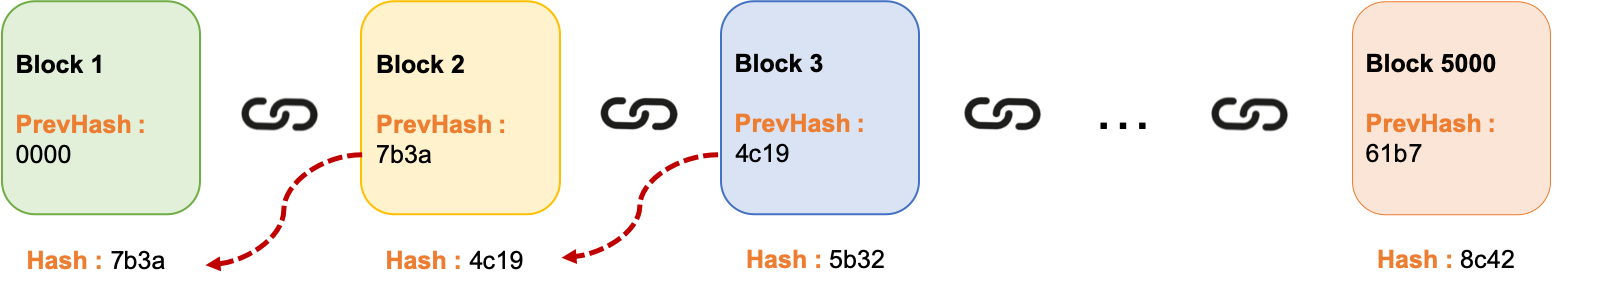
\includegraphics[width=0.9\textwidth]{img/hashchain.png}
	\caption{Hash chaining}
\end{figure}

To participate in the consensus process used to add more entries, a participant typically needs to know the current “state”, which is a function of all transactions ever executed. A new participant, or even a node that fell behind, can ask another node for the current state but it needs to download all the missing entries and recompute all the hashes up to the current entry to be sure that the obtained cumulative hash matches the obtained one. Even if there is some mechanism that allows to obtain a trusted current [???] without having to download all the entries, whenever the node wants to confirm historical transactions it needs to download all the entries between the transaction that it wants to confirm and the current one, and recompute all the hashes between them to confirm that the obtained cumulative hash matches the known one. 
This strategy can be very slow and expensive, depending on the size of the log - scalability problem.

\gls{aaosl} attempt to address this problem and are described following.

\subsection{Authenticated Append-Only SkipLists}
SkipLists  are sorted linked lists with extra links, designed to allow fast lookup of the stored elements by taking ``shortcuts''. Traditionally they are a probabilistic data structure, used as an alternative to binary search trees. The basic idea is to connect each element in the sequence not only with its successor, but also linking some elements to successors further down the sequence. This skip pointers are used to traverse the list achieving logarithmic traversal path lengths in the number of data elements \citep{pugh}.

\cite{skiplist} introduced the \gls{aaosl}, which take advantage of the shortcut idea, albeit in a deterministic way instead of the randomized version in the original skiplists. Conceptually, an \gls{aaosl} of n elements consist of $log_2\ n$ coexisting linked lists, each one with a different \textit{level} number. The linked list at level $0$ is a regular linked list connecting all elements in the data sequence. The linked list at level $l$ contains every $2^l$-th element of the original sequence. Thus, element $i$ belongs to the $l$-level linked list if and only if $i$ is divisible by $2^l$.


\begin{figure}[h]
    \centering
    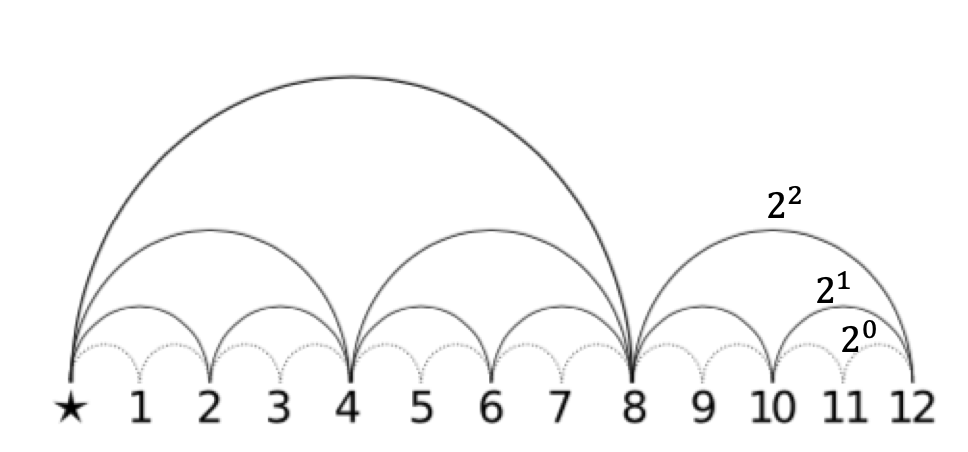
\includegraphics[width=0.53\textwidth]{img/skiplist1.png}
    \caption{SkipLog levels}
    \label{fig:levels}
\end{figure}

We can look at every index as having \textit{back skip pointers} per power of two (Figure \ref{fig:levels}). Suppose one wants to traverse the list from index 12 to index 4. The shortest path is to take the skip pointer at level $2$, from $12$ to $8$, then the one at level $2$, from $8$ to $4$. A skip pointer at level $l$ enables us to skip $2^l$ entries back. To know the maximum \textit{hop} level that we can take from a given index $i$ we need to know how many times $i$ is divisible by $2$, for instance, $12$ is divisible by $2$ twice, therefore the maximum hop that we can take from $12$ is $2^2$ entries back. 

In original SkipLists, the skip pointers are used to actually traverse the list, while in \gls{aaosl} the skip pointers work as a \textit{dependency graph} of the necessary entries to compute the actual entry. 
Index $0$ denotes the genesis block, $\star$, whose hash $h_\star $ is known to all participants. The level of a given index is exactly how many other indexes it depends on. 
Remember that in hash chaining every new entry that is appended to the log depends on the hash of the previous block. In \gls{aaosl}, however, the hash of the appended entry is computed, ensuring that it depends directly on every log entry one skip pointer away from it. Thus, the hash of log index 12 depends on 11, 10 and 8, which depends on 7, 6, 4, and $\star$.

\subsubsection{Advancement proofs}
As more data is appended to the log, clients must be convinced that history was not rewritten, that is, the history that the clients were aware of was taken into account when computing the new positions in the log. 

Assuming that Alice trusts $h_7$, the cumulative hash of position $7$, but has not verified that the log advanced from index $7$ to $12$. With the traditional hash chaining, an advancement proof consists only on the cumulative hash for position $12$. However to confirm that the history that she is aware of (up to position $7$) was taken into account, she needs to download and verify all the entries between $7$ and $12$ to confirm that the obtained cumulative hash matches the given hash for position $12$. With \gls{aaosl}, to prove to Alice that the advancement from $7$ to $12$ is consistent with the log up to index $7$ that she already trusts, we must provide enough information to enable Alice to construct $h_{12}$ from the hashes she already trusts. The advancement proof for Alice will consist in hashes $h_4$, $h_6$, $h_10$, $h_11$ and the hashes of the data in positions $12$ and $8$. With that she can build $h_12$ using her own hash for $7$ and $h_\star$ (Figure \ref{fig:deps}). Again, she needs to compare the obtained $h_12$ with the given one to confirm that the advancement proof was honest.

\begin{figure}[h]
    \centering
    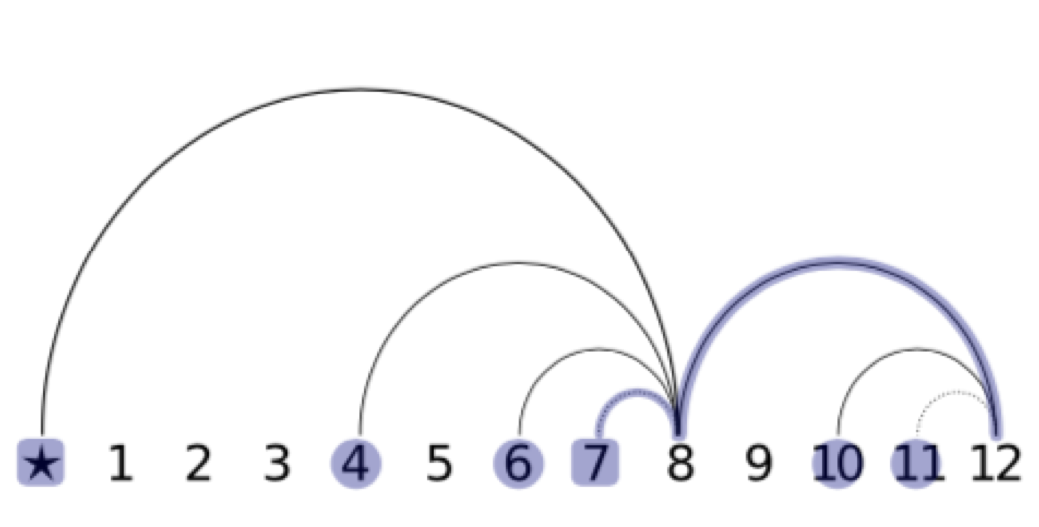
\includegraphics[width=0.5\textwidth]{img/skiplist2.png}
    \caption{Advancement proof from $7$ to $12$.
    Circles represent information verifier needs, squares represents information verifier already has, and the bold links show the path from 12 to 7}
    \label{fig:deps}
\end{figure}

\subsubsection{Membership Proof}
The advancement proof can also be used in the other ``direction''. Suppose, Alice already knows the expected value for $h_12$ (e.g., because consensus has been reached on it) but she wants to confirm the commited entry for position $7$, in other words, that entry $7$ is a member of the log. She will need the same information as in the advancement proof above together with the data for position $7$ - \textit{Membership proof}. In this case, she can compare her computed value for the cumulative hash of position $12$ with the $h_{12}$ she already trusted to confirm that the advancement from index $7$ to $12$ was honest.

\vspace{5mm}
To summarize, in \gls{aaosl} every entry in the log depends not only on the previous entry but also on previous entries in the log. As a result, to verify a given entry, a node only needs an advancement/membership proof which verification is logarithmic on the size of the log instead of linear as in the traditional hash chaining strategy.



\section{Consensus protocols}
%\subsection{Overview}

%pode ser usado na introdução
%The whole blockchain acts as a trusted system, it should be \textit{dependable}, \textit{resilient} and \textit{secure}, ensuring properties such as availability, reliability, safety, confidentiality, integrity and more.
Although a blockchain is maintained by multiple nodes that do not trust each other, the whole blockchain must act as trusted system. As such, all nodes must validate, in principle, the new entries to be appended to the log, simulating the trust of all nodes in that the blockchain as a whole operates correctly.

Blockchains operate in environments where network connectivity is uncertain, nodes may crash or behave maliciously, and interactions among nodes are inherently asynchronous. Therefore, blockchains can benefit from techniques developed for reaching consensus, replicating state, broadcasting transactions, etc. addressing many of the problems that have been studied in the field of distributed computing, most prominently for developing \gls{bft} systems \citep{wild}.

\begin{figure}
    \centering
    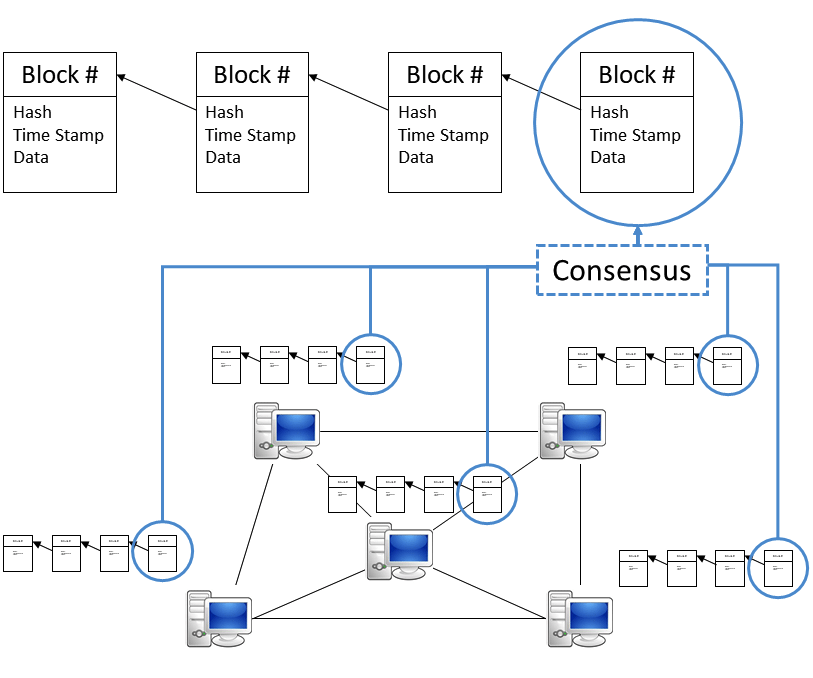
\includegraphics[width=0.7\textwidth]{img/Key-Elements-of-Blockchain-Systems.png}
    \caption{Consensus protocol in Blockchains \citep{blockchainConsensusImg}}
    \label{fig:blockchainConsensus}
\end{figure}


\subsection{Byzantine Fault Tolerant (BFT) protocols}
Historically, fault-tolerant protocols were meant to address common failures, such as crashes.  \cite{Lamport:1982:BGP:357172.357176} pioneered the formal study and development of algorithms for reaching consensus in the presence of failures, formulating the Byzantine Generals Problem where the term byzantine failure was coined. Byzantine Fault Tolerance refers to the ability of a system to endure arbitrary failures of its components. 
In the context of a blockchain, the \gls{bft} consensus protocol is used to limit the power of individual nodes in the system given that, not only they can crash or fail but some of this nodes may act maliciously against the common goal of reaching agreement.

%\subsubsection{Assumptions}
When assessing such protocols, it is important to be clear about the underlying trust assumptions specifying the environment for which the protocol is designed and in which it satisfies its guarantees. More concretely, the trust assumptions may include how many faulty nodes the protocol is resilient, the network model under which the protocol operates, the cryptographic assumptions of the cryptographic primitives used in the protocol, amongst others varying from different protocols. 

\vspace{3mm}
%\paragraph{Byzantine nodes}
The typical generic trust assumption for a system with $n$ independent nodes states that no more than $f < \displaystyle \frac{n}{k}$ nodes become faulty, for some $k = \{2, 3, ...\}$, the other $n - f$ nodes are correct. For instance, one of the most famous consensus algorithms is \textit{Paxos} \citep{Lamport:1998:PP:279227.279229,lamport2001paxos} , resilient to $ f < \displaystyle \frac{n}{2}$ node crashes. \textit{Raft} is a variant of this algorithm developed by \cite{Ongaro:2014:SUC:2643634.2643666} with the aim of simplifying the understanding and implementation of \textit{Paxos}. All protocols in this family progress in a sequence of \textit{views} or \textit{epochs}, with a unique leader per epoch that is responsible for progress. If the other nodes suspect that the leader has failed they elect a new leader moving to a new epoch. However, this family of protocols is resilient to byzantine failures in the classical meaning of the term, which is they are resilient to the crash of the nodes, but they are not resilient to actively dishonest nodes. For instance, a dishonest leader can easily convince two different nodes that two different transactions happened in the same log position. Despite that, it is important to mention them since they are the basis of most leader-based \gls{bft} algorithms up to date. 

\vspace{3mm}
%\paragraph{Network}
Regarding the network model, the first solution introduced by \cite{Pease:1980:RAP:322186.322188} relied on synchrony, a dependency that practical systems wish to avoid due to its complexity and also because it exposes the system to \gls{dos} attacks.
Later, \cite{Dwork:1988:CPP:42282.42283} introduced the \textit{eventual synchrony} model. It models a network that goes through transient periods of asynchrony , but eventually behaves synchronously. This protocol preserves safety during the asynchronous periods and, although it may stall during these periods, when the network stabilizes and behaves synchronously, then termination (\textit{liveness}) is guaranteed.
Formally, the eventually synchrony model assumes there is a known bound $\delta$ and an unknown \gls{gst}, such that after \gls{gst}, all transmissions between two correct replicas arrive within time $\delta$.

\citeauthor{Dwork:1988:CPP:42282.42283}'s approach underlies most practical \gls{bft} works to date. Specifically, it underlies the first practical solution introduced by \cite{Castro:1999:PBF:296806.296824} called \gls{pbft}. It can be understood as an extension of \textit{Paxos} in which a stable leader requires $O(n^2)$ communication and two round-trips per decision, and the leader replacement protocol incurs $O(n^3)$ communication. \gls{pbft} tolerates $f < \displaystyle \frac{n}{3}$ and has been deployed in several practical systems, some of them with variants aiming to optimize the cost. For instance, two blockchain systems, Tendermint \citep{DBLP:journals/corr/abs-1807-04938} and Casper \citep{DBLP:journals/corr/abs-1710-09437}, presented an optimized variant of \gls{pbft}.

Many of these practical solutions for \gls{bft} replication operate in a \textit{round by round} manner. There is a fixed mapping designating a \textit{leader} for each round. In each round the designated leader must broadcast a unique proposal for the round. The leader is successful if it can broadcast its proposal before honest validators time out and move to the next round. Usually these solutions operate in two phases per round. In the first phase (prepare), a quorum of validators \textit{certifies} (vote for) the proposal. In the second phase (commit), a quorum of validators vote for the certified proposal driving a \textit{commit} decision (Figure \ref{fig:pbft}). 

\begin{figure}[h]
\centering
    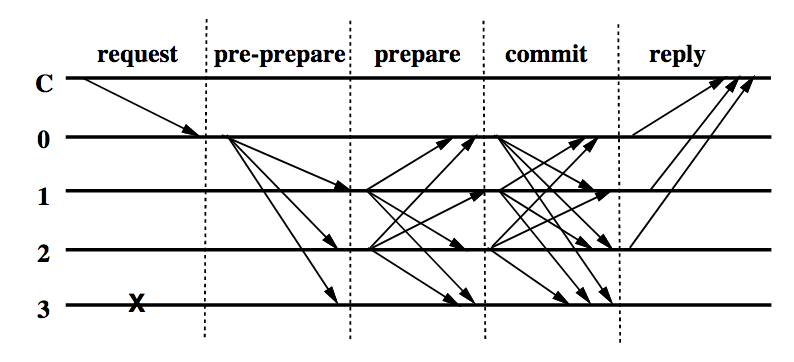
\includegraphics[width=0.7\textwidth]{img/pbft.png}
    \caption{\gls{pbft} normal operation. \\ $C$ is the client, node $0$ is the leader for the round and $3$ is faulty \citep{Castro:1999:PBF:296806.296824}}
    \label{fig:pbft}
\end{figure}

%\subsection{PBFT}

%\vspace{5mm}
With the growing popularity of blockchains, existing consensus protocols have received renewed attention for applying them to blockchain systems.  Over the recent years, many proposals for distributed ledger systems and completely new blockchain protocols have appeared. 

\subsubsection{HotStuff}

\textit{HotStuff} \citep{hotstuff} is one of the most recently published (PODC 2019) \gls{bft} consensus protocol. It is based on \gls{pbft} but it takes three phases to commit a decision. The first and the second phases of a round are similar to \gls{pbft}, but the result of the second phase is a certified certificate, rather than a commit decision, and the commit decision is reached upon getting a quorum of votes on the certified certificate.

HotStuff makes use of threshold signatures. In a $(k, n)$-threshold signature scheme, there is a single public key held by all replicas, and each of the $n$ replicas holds a distinct private key. Each replica can use its private key to contribute a partial signature on message $m$. A threshold of $k$ partial signatures can be combined to produce a digital signature on $m$. Any other replica can verify the signature using the public key.

\begin{figure}[h]
\centering
    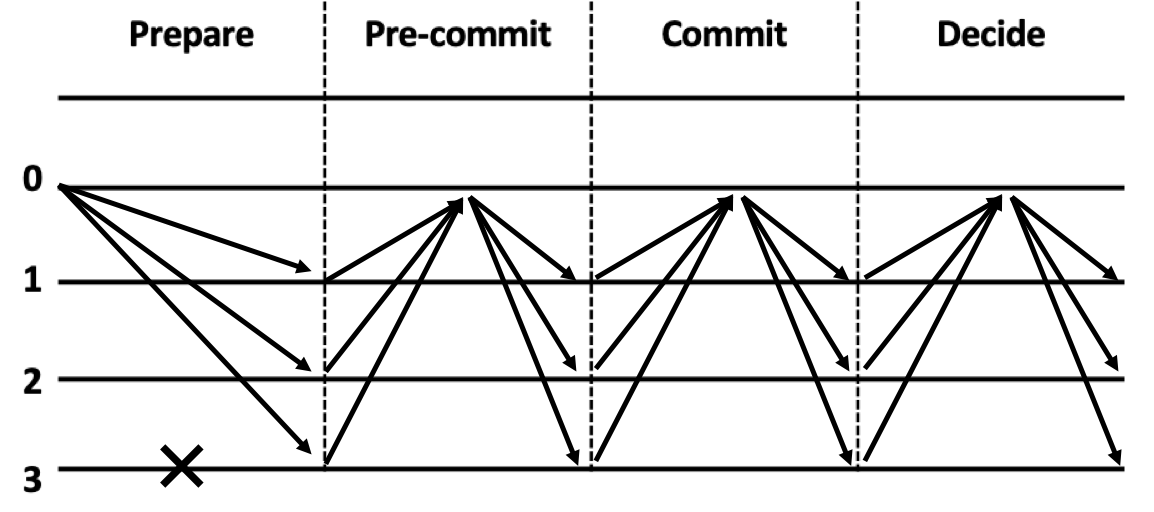
\includegraphics[width=0.7\textwidth]{img/hotStuff.png}
    \caption{Basic HotStuff normal operation.\\ 
    Node $0$ is the leader for the round, 3 is faulty}
    \label{fig:hotstuff}
\end{figure}

In each phase of HotStuff, only the leader broadcasts to all replicas while the replicas respond to the sender once with a partial signature to certify the vote. The complete signature is generated when the leader receives enough votes and constitutes a \gls{qc} for the current phase. The leader will attach this \gls{qc} to the message of the next phase and broadcast it to the replicas that verify the \gls{qc} is valid. With this scheme, HotStuff alleviates the need for all-all communication. Therefore, in each phase, there are $O(n)$ authenticators (partial signatures) received in total. As there is a constant number of phases, the overall complexity per view is $O(n)$.


%Explicar as fases fo HotStuff???

As all phases are similar and are not doing ``useful'' work except collect votes from replicas, HotStuff presented a chaining version of the basic protocol. In this version, the three phases for commitment are spread across rounds. The leader of round $v$ drives only a single phase of certification broadcasting the \gls{qc} for the proposal it made. The leader for round $v+1$ does not actually carry a pre-commit phase, but instead initiates a new prepare phase and adds its own proposal. This prepare phase for view $v+1$ simultaneously serves as the pre-commit phase for view $v$. The prepare phase for view $v+2$ simultaneously serves as the pre-commit phase for view $v+1$ and as the commit phase for view $v$. This is possible because all the phases have identical structure and reduces the number of message types and allows for pipelining of decisions. In figure \ref{fig:hotstuff-chain} we can observe that the command proposed by leader from $v_1$ would be made final at $v_4$.

\begin{figure}[h]
\centering
    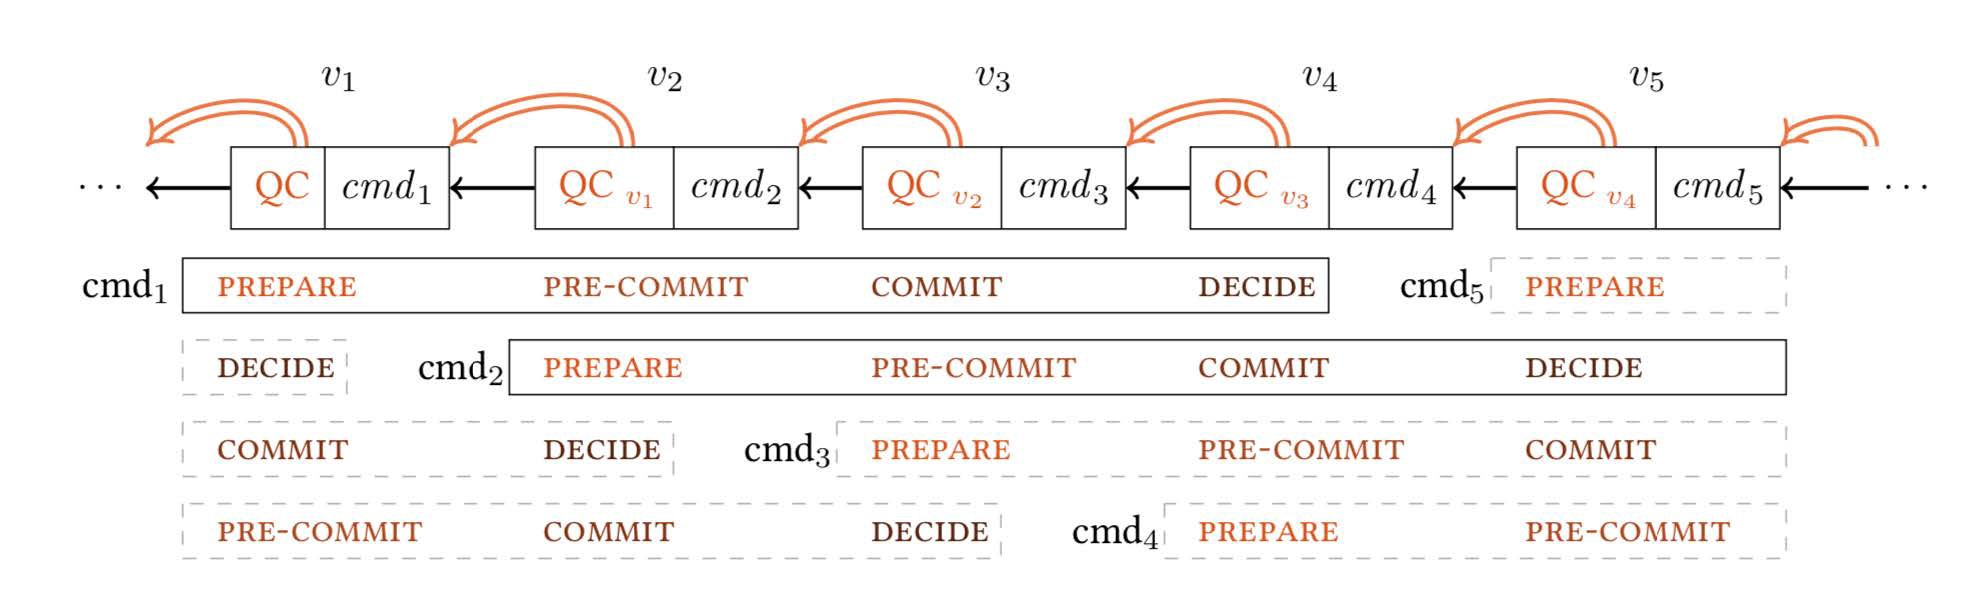
\includegraphics[width=1.0\textwidth]{img/hotstuff-chain.jpeg}
    \caption{Chained HotStuff is a pipelined Basic HotStuff where a QC can serve in different phases simultaneously \citep{hotstuff}}
    \label{fig:hotstuff-chain}
\end{figure}

HotStuff improves upon \gls{pbft} implementations and claims to be the first \gls{bft} protocol to achieve the following two properties together:

\begin{itemize}
    \item \textbf{Linear View Change:} After GST, any correct leader sends only $O(n)$ authenticators to drive a consensus decision, even when a leader is replaced. Consequently, communication costs to reach consensus after \gls{gst} is $O(n^2)$ authenticators in the worst case of cascading leader failures.
    \item \textbf{Optimistic Responsiveness:} After \gls{gst}, any correct leader needs to wait just for the first $n-f$ responses to guarantee that it can create a proposal that will make progress, even when a leader is replaced.
\end{itemize}

\subsection{LibraBFT}
\gls{lbft}, based on \textit{HotStuff}, is the \gls{bft} consensus protocol that is proposed for use in Facebook's emerging blockchain platform.


\section{Proving liveness}
\subsection{Conceptual map (Optional)}

%You may wish to use the \conexp{Concept-Explorer} tool.

    
    % CHAPTER - Problem and Challenges ---------------
	\chapter{The problem and its challenges}

"The problem with bad security is that it looks just like good security. You can’t tell the difference by looking at the finished product. Both make the same security claims; both have the same functionality. (...) Both might use the same protocols, implement the same standards, and have been endorsed by the same industry groups. Yet one is secure and the other is insecure." Schneier


%Pedaços de texto que posso usar mais tarde
"A resilient consensus protocol is only useful when it continues to deliver the intended service even under adversarial influence on the nodes and the network. Detailed analysis and formal argumentation are necessary to gain confidence that a protocol achieves its goal. In that sense, distributed consensus protocols resemble cryptosystems and other security mechanisms: they require broad agreement on the underlying assumptions, detailed security models, formal reasoning, expert judgement, open validation and wide spread public discussion. 

Verifying and establishing trust in the security, consistency and liveness semantics of a blockchain protocol is challenging.
A security solution should come with a clearly stated security model and trust assumption, under which the solution should satisfy its goal. This is widely accepted today; it prompts the question of how to validate that the solution satisfies its goal.

The experimental validation of a security solution in the information technology space fails very often because no experiment can exhaustively test the solution in all scenarios permitted by the model. In a way, experimentation can only demonstrate the failure of a security mechanism.

Therefore one needs to apply mathematical reasoning and formal tools to reason why the solution would remain secure under any scenario permitted by the stated trust assumption. Without such reasoning, security claims remain vague.

In a “provably secure” solution, an attack on the stated goal of the solution can be turned efficiently into a violation of some underlying assumption."
\citep{wild}







\iffalse

	         The problem and its challenges.

	\section{Proposed Approach - solution}
	In this section, it is presented various ways to display an image.
     \subsection{System Architecture}
     A block diagram of the planned system / approach

	Here we have an example of inserting an image between the text paragraphs.
	\begin{center}
		
\includegraphics[width=0.2\textwidth]{img/mei-logo-03.jpg}
	\end{center}

	\begin{wrapfigure}{r}{0.25\textwidth}	
		
\includegraphics[width=0.2\textwidth]{img/mei-logo-03.jpg}
	\end{wrapfigure}
	Here we have how an image can be wrapped into the text without having surronding space, and takin advantage of the space to be disposed on the side, without breaking the text readability.

	This approach also benefits from the fact that the text will be related implicitly to the image on its side, although the it should be referenced on the text anyway, otherwise, it should be consulting to perceive to which paragraph the image is related to.

	Here is how we place an image as floating body.
	Take in attention that the image is displayed on the next page, because there's no more room in this page.
	\begin{figure}
	\begin{center}
		
\includegraphics[width=0.5\textwidth]{img/mei-logo-03.jpg}
	\end{center}
	\caption{caption}
	\end{figure}



	You can also use an image as an icon, eg.~\href{http://mei.di.uminho.pt}{
\includegraphics[width=0.05\textwidth]{img/mei-logo-03.jpg}}, in the main tex.
	Click on it to visit the website. It is also listed in the list of terms.
	Another example of an item to appear in the term index: %\gls{um} (needs \Makeindex)
	
	\fi
	
	% CHAPTER - Contribution -------------------------
	\chapter{Development}
	\begin{lstlisting}
        lvlOf :: Index -> Level
        lvlOf 0 = 0
        lvlOf n = 1 + go n
            where go n = if even n then 1 + go (n `div` 2) else 0
    \end{lstlisting}

    We use the type synonyms Index and Level to make the role of these values evident, but these are all just Ints
    
	\section{Decisions}
    \section{Implementation}
    \section{Outcomes}
    Main result(s) and their scientific evidence
	\section{Summary}


	% CHAPTER - Application -------------------------
	\chapter{Case Studies / Experiments}
		Application of main result (examples and case studies)
	\section{Experiment setup}
    \section{Results}
    \section{Discussion}
	\section{Summary}

	% CHAPTER - Conclusion/Future Work --------------
	\chapter{Conclusion}
		Conclusions and future work.
	\section{Conclusions}
	\section{Prospect for future work}
			
	\bookmarksetup{startatroot} % Ends last part.
	\addtocontents{toc}{\bigskip} % Making the table of contents look good.
	%\cleardoublepage

	%- Bibliography (needs bibtex) -%
	\bibliography{dissertation}

	% Index of terms (needs  makeindex) -------------
	%\printindex
	
	
	% APPENDIX --------------------------------------
	\umappendix{Appendix}
	
	% Add appendix chapters
	\chapter{Support material}
	Auxiliary results which are not main-stream; or

	%\chapter{Details of results}
	Details of results whose length would compromise readability of main text; or

	%\chapter{Listings}
	Specifications and Code Listings: should this be the case; or

	%\chapter{Tooling}
	Tooling: Should this be the case.

	%Anyone using \Latex\ should consider having a look at \TUG,
	%the \tug{\TeX\ Users Group}


	% Back Cover -------------------------------------------
	\umbackcover{
	NB: place here information about funding, FCT project, etc in which the work is framed. Leave empty otherwise.
	}


\end{document}
